%% Except where otherwise noted, content in this documentation is Copyright (c)
%% 2015-2019, RTE (http://www.rte-france.com) and licensed under a
%% CC-BY-4.0 (https://creativecommons.org/licenses/by/4.0/)
%% license. All rights reserved.

\documentclass[a4paper, 12pt]{report}

% Latex setup
%%  Copyright (c) 2015-2019, RTE (http://www.rte-france.com)
%%  See AUTHORS.txt
%%  All rights reserved.
%%  This Source Code Form is subject to the terms of the Mozilla Public
%%  License, v. 2.0. If a copy of the MPL was not distributed with this
%%  file, you can obtain one at http://mozilla.org/MPL/2.0/.
%%  SPDX-License-Identifier: MPL-2.0
%%
%%  This file is part of Dynawo, an hybrid C++/Modelica open source time domain
%%  simulation tool for power systems.


%%%%%%%%%%%%%%%%%%%%%%%%%%%%%%%%%%%%%%%%%%%
% Define text and document settings
%%%%%%%%%%%%%%%%%%%%%%%%%%%%%%%%%%%%%%%%%%%

\usepackage{lmodern} % Latin Modern fam­ily of fonts
\usepackage[english]{babel} % English

% Specify encoding
\usepackage[utf8]{inputenc} % Input
\usepackage[T1]{fontenc} % Output

% Document structure setup
\usepackage{titlesec} % To change chapter format
\setcounter{tocdepth}{3} % Add subsubsection in Content
\setcounter{secnumdepth}{3} % Add numbering for subsubsection
\setlength{\parindent}{0pt} % No paragraph indentation

% Avoid numbering starting at each chapter for figures
\usepackage{chngcntr}
\counterwithout{figure}{chapter}

% Change title format for chapter
\titleformat{\chapter}{\Huge\bf}{\thechapter}{20pt}{\Huge\bf}

% To add links on page number in Content and hide red rectangle on links
\usepackage[hidelinks, linktoc=all]{hyperref}
\usepackage[nottoc]{tocbibind} % To add biblio in table of content
\usepackage{textcomp} % For single quote
\usepackage{url} % Allow linebreaks in \url command
\usepackage{listings} % To add code samples

% Define typography
\usepackage{xspace}
\usepackage{dirtree}
\newcommand{\Dynawo}[0]{Dyna$\omega$o\xspace}

% Default listings parameters
\lstset
{
  aboveskip={1\baselineskip}, % A bit of space above
  backgroundcolor=\color{shadecolor}, % Choose the background color
  basicstyle={\ttfamily\footnotesize}, % Use font and smaller size \small \footnotesize
  breakatwhitespace=true, % Sets if automatic breaks should only happen at whitespace
  breaklines=true, % Sets automatic line breaking
  columns=fixed, % Nice spacing -> fixed / flexible
  mathescape=false, % Escape to latex false
  numbers=left, % Where to put the line-numbers
  numberstyle=\tiny\color{gray}, % The style that is used for the line-numbers
  showstringspaces=false, % Do not emphasize spaces in strings
  tabsize=4, % Number of spaces of a TAB
  texcl=false, % Activates or deactivates LaTeX comment lines
  upquote=true % Upright quotes
}

%%%%%%%%%%%%%%%%%%%%%%%%%%%%%%%%%%%%%%%%%%%
% Define plots settings
%%%%%%%%%%%%%%%%%%%%%%%%%%%%%%%%%%%%%%%%%%%

% Macro pack­age for cre­at­ing graph­ics
\usepackage{tikz}
\usepackage{subfigure}
\usepackage{float}

% Draws func­tion plots (based on pgf/tikz)
\usepackage{pgfplots}
\pgfplotsset{enlarge x limits=false, xlabel={\begin{small}$time$ (s)\end{small}}, height=0.6\textwidth, width=1\textwidth}
\pgfplotstableset{col sep=semicolon}

% Define colors
\usepackage{color}
\definecolor{blue}{rgb}{.3,.5,1}
\definecolor{deepblue}{rgb}{0,0,1}
\definecolor{darkblue}{rgb}{0,0,.4}
\definecolor{red}{rgb}{1,0,0}
\definecolor{darkred}{rgb}{.56,0,0}
\definecolor{pink}{rgb}{.933,0,.933}
\definecolor{purple}{rgb}{0.58,0,0.82}
\definecolor{green}{rgb}{0.133,0.545,0.133}
\definecolor{darkgreen}{rgb}{0,.4,0}
\definecolor{gray}{rgb}{.3,.3,.3}
\definecolor{darkgray}{rgb}{.2,.2,.2}
\definecolor{shadecolor}{gray}{0.925}

%%%%%%%%%%%%%%%%%%%%%%%%%%%%%%%%%%%%%%%%%%%
% Define blocks for simple network drawings
%%%%%%%%%%%%%%%%%%%%%%%%%%%%%%%%%%%%%%%%%%%

% Define blocks for newtorks drawings
\usepackage{amsmath} % Add math­e­mat­i­cal fea­tures
\usepackage{schemabloc} % Add block diagram library (french one)

%% Define infinite bus
\tikzset{infinite bus/.pic={
  code={
  \draw (0,0) circle (2) node[inner sep=0, outer sep=0] {{$\infty$}};
  \draw (2,0) --++ (2,0);
  }
  }
}

%% Define transformer
\tikzset{transfo/.pic={
  code={
  \draw (0,0) circle (2);
  \draw (2,0) circle (2);
  \draw (4,0) --++ (4,0);
  \draw (-2,0) --++ (-4,0);
  }
  }
}

%% Define generator
\tikzset{generator/.pic={
  code={
    \draw (0,0) circle (2);
    \draw (0,0) arc (0:180:0.5);
    \draw (0,0) arc (180:360:0.5);
    \draw (-2,0) --++ (-2,0);
  }
  }
}

%% Define generator controls
\tikzset{VR/.pic={
  code={
  \draw (0,0) circle (2) node[inner sep=0, outer sep=0] {{VR}};
  }
  }
}

%% Define SVarC
\tikzset{SVarC/.pic={
  code={
  \draw (0,0) circle (4) node[inner sep=0, outer sep=0] {{SVarC}};
  }
  }
}


\begin{document}

\title{Configure \Dynawo}
\date\today

\maketitle
\tableofcontents

\chapter[Configure Dynawo]{Configure \Dynawo}

\section{Overview}

The following section will provide information on:
\begin{itemize}
\item How to create the input files in order to simulate a given test case;
\item How to configure the input files in order to get the  necessary output files to analyse the obtained results;
\end{itemize}

The list of input files and the most important output files are summarized in the figure below:

\begin{figure}[h!]
\centering
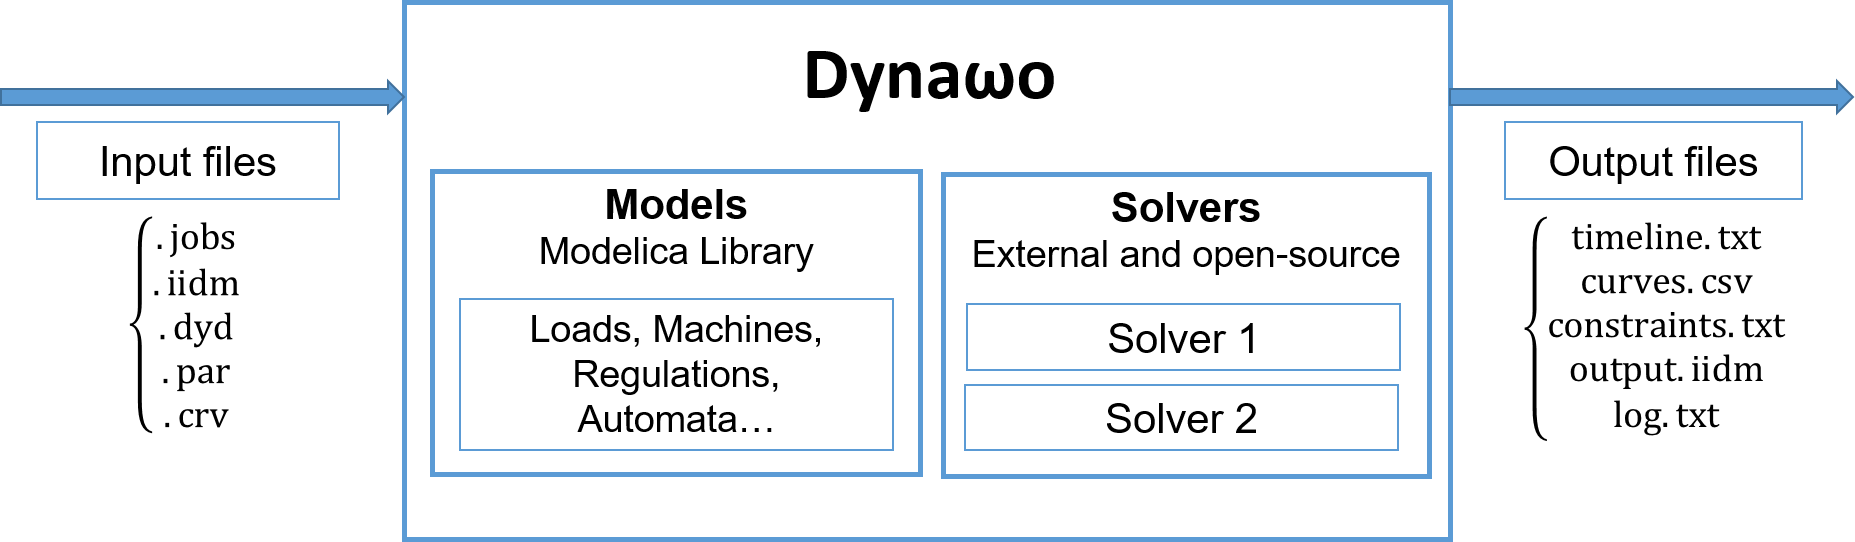
\includegraphics[width=\textwidth]{../resources/DynawoModelSolver.png}
\caption{\Dynawo input and output files}
\end{figure}

\subsection[Dynawo inputs]{\Dynawo inputs}

To run a simulation, \Dynawo needs most of the time five input files:
\begin{itemize}
\item A file providing the simulation settings: the jobs file (\textbf{.jobs} extension);
\item A file providing the static description of the test grid to simulate: the iidm file (\textbf{.iidm} extension);
\item A file providing the dynamic description of the test grid to simulate: the dynamic data file (\textbf{.dyd} extension);
\item A file providing the needed parameters of the simulation: the parameter file (\textbf{.par} extension);
\item A file providing the list of the variables to plot at the end of the simulation: the curves file (\textbf{.crv} extension);
\end{itemize}
The crv file is optional: with no crv file, no curves will be available at the end of the simulation but the simulation can be run anyway. The iidm file can also be optional for small test cases where the whole system is represented in the dyd file (see paragraph \ref{sec:Run a simulation with no iidm file}). Other files are mandatory. \\

All jobs, iidm, dyd, par and crv files are XML files. Their extension can also be .xml. For each file, there is an associated xsd file used to validate the xml file and to check that it respects a certain format. The xsd file defines which elements and attributes are permitted and in which order. In that sense, they can help the user write or modify one or several input files. The different xsd files are to be found in the install directory in \path{dynawo/share/xsd}.

\begin{itemize}
\item jobs.xsd for the jobs file;
\item dyd.xsd for the dyd file;
\item parameters.xsd for the par file;
\item curvesInput.xsd for the crv file;
\end{itemize}

The iidm.xsd is directly located in the install directory of the IIDM library and can be found in \path{share/iidm/xsd}.

\subsection[Dynawo outputs]{\Dynawo outputs}

After a simulation that went well, \Dynawo generates the following output files:
\begin{itemize}
\item A file providing the chronological list of events that happened during the simulation: component connection, disconnection, automata activation, etc (timeline.txt).
\item A file providing the list of constraints that happened in the network during the simulation (constraints.txt);
\item A file providing the static state of the network at the end of the simulation (output.iidm). This iidm file can be used to start another dynamic simulation;
\item A file providing the value of the desired variables at each time step in order to visualize their evolution through time (curves.crv);
\item A file providing information about how the simulation went (dynamo.log). This log file contains error messages if the simulation crashed;
\item Files providing the variables values after initialization for each model. The values can be printed after local (or individual model) initialization or global (or system) initialization.
\end{itemize}

The input jobs file should be configured properly in order to give access to all these outputs (see paragraph \ref{sec:Configure the jobs outputs}).

\section[Dynawo input files]{\Dynawo input files}

The following sections get into more details regarding the five input files and give some examples based on the non regression test IEEE14 present in the \Dynawo repository. \\
Warning: the following example files are extracted from IEEE14 case in \Dynawo and might not be complete, hence not work as they are presented here.

\subsection{jobs file}

The jobs file gathers information about the solver to use, the models to use, the simulation characteristics and the outputs wanted.

Here is an example on a jobs file:
\lstinputlisting[language=XML, morekeywords={solver, modeler, simulation, outputs},title=jobs file example]{../resources/syntaxExample/syntaxExample.jobs}

In this example, we want to simulate a 100 second scenario on IIDM network
IEEE14.iidm described by dynamic models included in IEEE14.dyd with a precision
of $10^{-6}$. A criteria file with stop conditions has been specified.
The models compiled by \Dynawo will be exported in \path{outputs/compilation} directory. Network parameters are stored in IEEE14.par file, set 18. \\

The solver used is the simplified solver, and its parameters are described in solvers.par file, set 1. \\

At the end of the simulation, the user will have the possibility to plot the different variables listed in IEEE14.crv, thanks to a csv file generated by \Dynawo in \path{outputs/curves} directory. \\

The chronology of events that happened during the simulation will also be available in a text file in \path{outputs/timeline} directory.

Absolute and relative paths can be used and mixed in a single jobs file. Relative paths refer to the directory where the jobs file is located.

\subsection{iidm file}

The iidm file represents the network to simulate with a static representation: it lists all the components present in the network and how they are connected. \\

Basically, the iidm file is composed of:
\begin{itemize}
\item the substations, which contain one or more voltage levels, which themselves contain buses, loads, generators, etc;
\item the branches (lines and transformers) that connect buses defined in the voltage levels;
\end{itemize}

Here is an example of an iidm file (extraction from IEEE14.iidm):
\lstinputlisting[language=XML, morekeywords={voltageLevel, line, bus, switch, load, generator, bus1, bus2}, title=iidm file example]{../resources/syntaxExample/syntaxExample.iidm}

In this example, the network is composed of only two voltage levels connected through one line. \\

The first voltage level (\_BUS\_\_\_10\_VL) has one bus (\_BUS\_\_\_10\_TN) and one load (\_LOAD\_\_10\_EC). The second voltage level (\_BUS\_\_\_11\_VL) has also one bus (\_BUS\_\_\_11\_TN) and one load (\_LOAD\_\_11\_EC). \\

The line connects the bus \_BUS\_\_\_10\_TN of voltage level \_BUS\_\_\_10\_VL and the bus \_BUS\_\_\_11\_TN of the voltage level \_BUS\_\_\_11\_VL. \\

iidm files are very dense and can be very large in case of large systems because they provide a lot of information:
\begin{itemize}
\item the \textbf{static parameters} with their values. For example, for the line the static parameters are: the resistance (R), the reactance (X), the conductances on both sides (G1, G2) and the susceptances on both sides (B1, B2).  They are used by \Dynawo to build the network model.
\item the \textbf{load flow outputs} obtained thanks to another simulation module: the voltages amplitude and angle at each bus (V, $\theta$) and the active and reactive power at each injection point: (P, Q) for the load in this example. They are used by \Dynawo to initialize the dynamic simulation.
\item the \textbf{network topology} in the initial situation. We have seen in our example that we have information about the connection between different voltage levels through a line.
\end{itemize}

\subsection{dyd file}

The dyd file gathers the dynamics models to use with their characteristics and if needed, their connections. \\

Here is an example of a dyd file (extraction from IEEE14.dyd):
\lstinputlisting[language=XML, morekeywords={modelicaModel,  blackBoxModel, connect}, title=dyd file example]{../resources/syntaxExample/syntaxExample.dyd}

In this example, we have two dynamic models: load \_LOAD\_\_10\_EC and load \_LOAD\_\_11\_EC. \\

The connections between these models are written at the end of the file: the load output terminal is connected to the pin of a bus given in the iidm file. The connections between the dynamics models are provided with the keyword ``connect''. \\

Here the load models are precompiled black-box models but the dyd file can use other kind of models such as macro Modelica models assembling different unit Modelica models, or template models. See following sections for more information about the different types of models supported by the dyd file. \\

In most cases, the iidm file provides information about the network topology and the static parameters, and the dyd file provides information about the dynamic behaviour of components given in the iidm file. \\

When a static component has no equivalent in the dyd file, \Dynawo uses a default C++ model for the component. This is often the case for the lines for example. It can also be the case for any other component, but the reader should keep in mind that the default C++ models are basic and simple models. In order to obtain accurate and detailed results from a dynamic simulation, it is important to use accurate and detailed models.

\subsection{par file}

The par file contains all the parameters for the simulation: the solver parameters and the dynamic models' parameters. All these parameters are gathered in sets. \\

Here is an example of a par file (extraction from IEEE14.par):
\lstinputlisting[language=XML, morekeywords={id, par, reference}, deletekeywords={type}, title=par file example]{../resources/syntaxExample/syntaxExample.par}

For each parameter, the user should give the name, the type (DOUBLE, INT, BOOL or STRING) and the value of the parameter. \\

Sometimes, the par file contains references to parameters present in the iidm file (see paragraph \ref{sec:Set a reference to a value stored in the iidm file}).

\subsection{crt file}

The crt file contains all the criteria files to be checked during the
simulation.
\\

Here is an example of a crt file :
\lstinputlisting[language=XML, morekeywords={criteria, parameters, component,
busCriteria, loadCriteria, generatorCriteria}, deletekeywords={type}, title=crt
file example]{../resources/syntaxExample/criteria.crt}

There are three different kind of criteria, depending on which type of component
is targeted.

Each criteria is then associated to an id, a set of parameters and optionally a list of component.

The scope of a criteria (specified in its parameters) can be one of 'DYNAMIC' if
the criteria should be checked at every time step or 'FINAL' if the criteria
should be respected only at the final step.

An empty component list means that all the component corresponding to the specified type will be subject to this
criteria. If some components id are specified then only those components will be subject to this
criteria. Components from the list should have the same type as the
specified type (buses, loads or generators).

\subsubsection{bus Criteria}

Bus criteria should have at least one of $UMinPu$ or $UMaxPu$ specified. Only
local values can be checked (parameter type = 'LOCAL\_VALUE').
It fails when the following condition happens for any of the bus: \\
\begin{center}
$U_{bus} < UMinPu*U_n$\\
and/or\\
$U_{bus} > UMaxPu*U_n$ \\
\end{center}
the buses taken into account are the ones that satisfy the
following condition:
\begin{center}
$UMaxNom \ge U_n \ge UMinNom$\\
\end{center}

$UMinNom$ and $UMaxNom$ are optionals. If one of them is not
specified, the corresponding condition is not applied.

\subsubsection{load and generators Criteria}

Load or generator (generically named source below) criteria should have at least
one of $PMin$ or $PMax$ specified.
If local values was selected  (parameter type = 'LOCAL\_VALUE'), it fails when
the following condition happens for any of the source:\\
\begin{center}
$P_{source} < PMin$\\
and/or\\
$P_{source} > PMax$\\
\end{center}
If sum was selected  (parameter type = 'SUM'), it fails when the
following condition happens: \\
\begin{center}
$\sum P_{source} < PMin$\\
and/or\\
$\sum P_{source} > PMax$ \\
\end{center}
In both cases, the sources taken into account are the ones that satisfy the
following conditions:\\
\begin{center}
$UMaxNom \ge U_n \ge UMinNom$\\
and\\
$UMaxPu*U_n \ge U_{source} \ge UMinPu*U_n$ \\
\end{center}

$UMinNom$, $UMaxNom$, $UMinPu$ and $UMaxPu$ are optionals. If one of them is not
specified, the corresponding condition is not applied.

\subsection{crv file}

The curves file lists all variables or parameters to plot. \\

Here is an example of a crv file (extraction from IEEE14.crv):
\lstinputlisting[language=XML, morekeywords={id},title=crv file example]{../resources/syntaxExample/syntaxExample.crv}

In this example, the curves available are the voltage amplitudes of buses \_BUS\_\_\_10\_TN and \_BUS\_\_\_10\_TN in per unit.

\section[Dynawo input files modification]{\Dynawo input files modification}

\Dynawo input files (jobs, iidm, dyd, par and crv) have been briefly described in the previous section. This section aims at giving more details on each file in order to help the user parametrize its inputs easily and autonomously.

\subsection{jobs file}

\subsubsection{Simulate several scenarios}

A jobs file can contain several jobs. For each job, the description is the same as illustrated in the previous section. The different jobs can be listed in the jobs file as in the example bellow:

\begin{lstlisting}[language=XML, morekeywords={name}]
<jobs xmlns="http://www.rte-france.com/dynawo">
  <job name="MyFirstJOB">
    ...
  </job>
  <job name="MySecondJOB">
    ...
  </job>
</jobs>
\end{lstlisting}

\subsubsection{Change the solver}

The jobs file specifies the solver library to use for the simulation. In \Dynawo two solvers are available:
\begin{itemize}
\item the simplified solver (fixed time step solver): library dynawo\_SolverSIM.so;
\item the IDA solver (variable time step solver): library dynawo\_SolverIDA.so;
\end{itemize}

For IDA solver, IDA order 1 and IDA order 2 can be used (fill the value for the parameter ``order'' in the par file).

\begin{lstlisting}[language=XML, morekeywords={lib}]
<job name="MyJOB">
  <solver lib="dynawo_SolverIDA.so" parFile="MyPAR.xml" parId="0"/>
  ...
</job>
\end{lstlisting}

The solver library is stored in the install directory in \path{dynawo/lib}.

\subsubsection{Specify stop conditions for the simulation}

The jobs file specifies the following simulation settings:
\begin{itemize}
\item the start time of the simulation;
\item the stop time of the simulation;
\item the list of criteria to check;
\end{itemize}

When no criteria is specified, simulation will stop at the stop time given by
the user. Otherwise, the simulation could stop before the stop
time if a criteria is not respected.

\begin{lstlisting}[language=XML, morekeywords={activateCriteria}]
<job name="MyJOB">
  ...
  <simulation startTime="0" stopTime="100" precision="1e-6">
    <criteria criteriaFile="criteria.crt"/>
  </simulation>
  ...
</job>
\end{lstlisting}

\subsubsection{Specify what kind of models to use}

Dynamic models used by \Dynawo are either precompiled models or Modelica models. The user should specify which kind of models he wants to use (he can use both). These items may have an additional ``directory'' attribute with the path to case-specific models.

\begin{lstlisting}[language=XML, morekeywords={precompiledModels, modelicaModels}]
<job name="MyJOB">
  ...
  <modeler compileDir="outputs/compilation">
      ...
      <precompiledModels useStandardModels="true"/>
      <modelicaModels directory="MyDirectory" useStandardModels="true"/>
  </modeler>
  ...
</job>
\end{lstlisting}

\subsubsection{Start a simulation from the end of another one}

In order to start a simulation from the end of another simulation, the item ``initialState'' should be added in the modeler section of the job file. The name of the dumpFile should be specified. This binary file contains the values of all variables and their derivatives at the end of the previous simulation and is needed to initialize the new simulation at the same operating point that the end of the previous simulation. To obtain this file, use the finalState item of the outputs section (see paragraph \ref{sec:Configure the jobs outputs}).

\begin{lstlisting}[language=XML, morekeywords={initialState}]
<job name="MyJOB">
  ...
  <modeler compileDir="outputs/compilation">
      <dynModels dydFile="MyDyd.dyd"/>
      <initialState file="dumpFile"/>
      ...
  </modeler>
  ...
</job>
\end{lstlisting}

\subsubsection{Run a simulation with no iidm file}
\label{sec:Run a simulation with no iidm file}

It is not mandatory to provide the jobs file with an iidm file as long as the whole system is described in the dyd file. We use this technique for small test cases such as unitary test cases with a few number of components. In that case, all models are listed in the dyd file, as well as all connections. Static components and topology normally defined in the iidm file should consequently be defined in the dyd file (buses, lines, etc).

\subsubsection{Configure the jobs outputs}
\label{sec:Configure the jobs outputs}

The user can specify in the jobs file what outputs he wants to get from the simulation. The outputs are to be found in the jobs file directory or in a user-chosen directory when the attribute ``directory'' is provided:

\begin{lstlisting}[language=XML,numbers=none]
<outputs directory="outputs/">
\end{lstlisting}

Several outputs are available with \Dynawo:
\begin{itemize}
\item \textbf{Initialization}: the user can have access to the results of the initialization stages (local and/or global) by adding the item ``dumpInitValues'' in the jobs file.

\begin{lstlisting}[language=XML, morekeywords={dumpInitValues},numbers=none]
<dumpInitValues local="true" global="true"/>
\end{lstlisting}

\item \textbf{Constraints}: the user can have access to the list of constraints that happened during the simulation by adding the item ``constraints'' in the jobs file, and by specifying the export mode.
\begin{lstlisting}[language=XML, morekeywords={constraints},numbers=none]
<constraints exportMode="TXT"/>
\end{lstlisting}
Two export modes are available for constraints: TXT or XML.

\item \textbf{Timeline}: the user can have access to the list of events that happened during the simulation and the instant of their occurrence by adding the item ``timeline'' in the jobs file, and by specifying the export mode.

\begin{lstlisting}[language=XML, morekeywords={timeline},numbers=none]
<timeline exportMode="TXT"/>
\end{lstlisting}
Three export modes are available for the timeline: TXT, XML or CSV.

\item \textbf{Final state}: the user can have access to the final state of the simulation thanks to two files: the iidm file and the dump file. The user can specify which of those he wants to obtain. The iidm output file contains the static data of the network at the end of the simulation. The dump file is a binary file that contains the value of all dynamic variables and derivatives at the end of the simulation and that enables to restart another simulation from this operating point.

\begin{lstlisting}[language=XML, morekeywords={finalState},numbers=none]
<finalState exportIIDMFile="true" exportDumpFile="true"/>
\end{lstlisting}

\item \textbf{Curves}: the user can plot curves at the end of the simulation. To do so, he should specify the name of the file containing the list of the variables to be plotted and the export mode.
\begin{lstlisting}[language=XML, morekeywords={curves},numbers=none]
<curves inputFile="MyCurves.crv" exportMode="CSV"/>
\end{lstlisting}
Two export modes are available for curves export: CSV or XML.

\item \textbf{Logs}: the user can have access to different log files that give information about the execution of the compilation and the simulation, and that could help him in case of failure. The main log file corresponds to the appender with no tag named ``dynawo.log'' in the example below.
\begin{lstlisting}[language=XML, morekeywords={logs}]
<logs>
  <appender tag="" file="dynawo.log" lvlFilter="DEBUG"/>
  <appender tag="NETWORK" file="network.log" lvlFilter="DEBUG"/>
  <appender tag="MODELER" file="modeler.log" lvlFilter="DEBUG"/>
  <appender tag="COMPILE" file="compile.log" lvlFilter="DEBUG"/>
  <appender tag="PARAMETERS" file="param.log" lvlFilter="DEBUG"/>
  <appender tag="VARIABLES" file="variables.log" lvlFilter="DEBUG"/>
  <appender tag="EQUATIONS" file="equations.log" lvlFilter="DEBUG"/>
</logs>
\end{lstlisting}

For each ``appender'', a format could be configured to set how the log should be printed. By default, the format of the ``appender'' is the following:
\begin{lstlisting}[numbers=none]
%Y-%m-%d %H:%M:%S | <lvlFilter> | log
\end{lstlisting}

where ``lvlFilter'' is used to filter the trace exported by giving the minimum level exported. For example, if a level filter of ``WARN'' is set, only logs declared as ``WARN'' or ``ERROR'' will be exported. \\

The available filters are: DEBUG, INFO, WARN, ERROR.
\end{itemize}

\subsection{dyd file}

Different types of dynamic models can be used by \Dynawo and specified in the dyd file:
\begin{itemize}
\item Black-box models;
\item Modelica models;
\item Template models;
\end{itemize}

The following subsections explain how to use these models and how to write the dyd file in the different cases.

\subsubsection{Use a black-box model}

Black box models are precompiled black-box libraries. In order to use a black box model, the user should specify the model library, the associated par file and the parameters' set.
\begin{lstlisting}[language=XML, morekeywords={lib},numbers=none]
<blackBoxModel id="Model" lib="MODEL_LIB.so" parFile="MyPar.par" parId="5">
\end{lstlisting}

The models libraries are stored in the install directory in \path{dynawo/ddb}.

\subsubsection[Use a Modelica model from Dynawo library]{Use a Modelica model from \Dynawo library}

Several Modelica models are included in the \Dynawo Modelica library. Most of the time, the Modelica models used by the dynamic simulation are present in this library. To use one of these models, the user should specify the name of the dynamic and the init models in the Modelica library, the associated par file and the parameters' set.

\begin{lstlisting}[language=XML, morekeywords={name, initName}]
<modelicaModel id="MacroModel">
  <unitDynamicModel id="Model1" name="Model1" initName="Model1_INIT" parFile="MyPar.par" parId="2"/>
</modelicaModel>
\end{lstlisting}

The name of the model should include the whole path through the library, for example for a transformer: Dynawo.Electrical.Branches.Transformer.

\subsubsection[Use a Modelica model not in Dynawo Library]{Use a Modelica model not in \Dynawo Library}

To use a Modelica model that is not in the library, the user should provide the path to the dynamic and the init models to use. To do so, two attributes should be added to the ``unitDynamicModel'' item: ``moFile'' and ``initFile''.

\begin{lstlisting}[language=XML, morekeywords={moFile, initFile}]
<modelicaModel id="MacroModel">
  <unitDynamicModel id="MyModel" name="MyModel" moFile="myDirectory/MyModel.mo" initFile="myDirectory/MyModel_INIT.mo" parFile="MyPar.par" parId="1"/>
</modelicaModel>
\end{lstlisting}

\subsubsection{Assemble unit Modelica models in a macro model}

In the dyd file, several ``unitDynamicModel'' can be assembled to build a macro model. To define a macro model, the user should list in the ``modelicaModel'' section the different ``unitDynamicModel'' present and their connections. The connections between the dynamic models are provided with the keyword ``connect'', and the connections between the initialization models are provided with the keyword ``initConnect"".

\begin{lstlisting}[language=XML, morekeywords={unitDynamicModel, connect, initConnect}]
<modelicaModel id="MacroModel">
  <unitDynamicModel id="Model1" name="Model1" initName="Model1_INIT" parFile="MyPar.par" parId="2"/>
  <unitDynamicModel id="Model2" name="Model2" initName="Model2_INIT" parFile="MyPar.par" parId="3"/>
  <connect id1="Model1" var1="var1" id2="Model2" var2="var1"/>
  <initConnect id1="Model1" var1="var1" id2="Model2" var2="var1"/>
</modelicaModel>
\end{lstlisting}

We use this technique for example to assemble the physical model of a generator with the models of its regulations: the result is a macro model of a generator with its controllers.

\subsubsection{Use a template model}

Template model enables the user to define a macro model thanks to unit Modelica models (see section "How to assemble unit Modelica models in a macro model").

\begin{lstlisting}[language=XML]
<modelTemplate id="Template">
 <!-- insert here any unitDynamicModel, connect, initConnect... -->
\end{lstlisting}

The template is instantiated as:
\begin{lstlisting}[language=XML,numbers=none]
<modelTemplateExpansion id="TemplateModel" templateId="Template" parFile="MyPar.par" parId="6">
\end{lstlisting}

\subsubsection{Write connections}

The connections between the dynamics models are provided with the keyword ``connect'', and the connections between the initialization models are provided with the keyword ``initConnect''.
\begin{lstlisting}[language=XML]
<connect id1="id1" var1="var1" id2="id2" var2="var1"/>
<initConnect id1="id1" var1="var1" id2="id2" var2="var1"/>
\end{lstlisting}

Here are a few rules to follow to write models connections:
\begin{itemize}
\item When connecting to the AC network (C++ model), the id to use is ``NETWORK'';
\item For connections between precompiled models, id1 and id2 refer to the models id and var1 and var2 are simply the variables name;
\item For connections between unit Modelica models in a macro model, id1 and id2 refer to the unit models id and var1 and var2 are simply the variables name;
\item For connections between macro Modelica models, id1 and id2 refer to the macro models id and var1 and var2 should be built as:

\verb|unitModelId_VariableNameInModel|;
\end{itemize}

\subsubsection{Associate a dynamic model to a static component}

When an iidm file is used, a correspondence between the component in the iidm file and its dynamic equivalent in the dyd file is made thanks to the item ``staticId''.
\begin{lstlisting}[language=XML, morekeywords={staticId}]
<modelicaModel id="MyModel" staticId="MyModelIIDMId">
  ...
  <staticRef var="DynVarName" staticVar="StaticVarName"/>
</modelicaModel>
\end{lstlisting}

Static references may be defined in order to describe which dynamic variables may be used to update the iidm output file. Static references are often defined for active and reactive power. Here is an example:
\begin{lstlisting}[language=XML, morekeywords={staticRef}]
<modelicaModel id="MyGenerator" staticId="MyGeneratorIIDMId">
  ...
  <staticRef var="P_value" staticVar="p"/>
  <staticRef var="Q_value" staticVar="q"/>
  <staticRef var="state" staticVar="state"/>
</modelicaModel>
\end{lstlisting}

If no static references are done, the simulation will proceed but \Dynawo will not be able to output an iidm file.

\subsubsection{Define sets of connections}

The connection between two different dynamic models in the dyd file often needs more than one ``connect'' statement. For example,  in order to connect the reference frequency model to a generator model we need to connect three variables: omega, omegaRef, running. In order not to write the three connections for each generator model of the network, we can define a macro connection in the dyd file:
\begin{lstlisting}[language=XML, morekeywords={macroConnector}]
<macroConnector id="M1S_OMEGAREF_CONNECTOR">
  <connect var1="omega_grp_@INDEX@" var2="M1S_omega"/>
  <connect var1="running_grp_@INDEX@" var2="M1S_running"/>
  <connect var1="omegaRef_grp_@INDEX@" var2="M1S_omegaRef"/>
</macroConnector>
\end{lstlisting}

And then we can use this macro connection as many time as needed with the keyword ``macroConnect'':
\begin{lstlisting}[language=XML, morekeywords={macroConnect}]
<macroConnect connector="M1S_OMEGAREF_CONNECTOR" id1="MODEL_OMEGA_REF" index1="0" id2="Generator0"/>
<macroConnect connector="M1S_OMEGAREF_CONNECTOR" id1="MODEL_OMEGA_REF" index1="1" id2="Generator1"/>
<macroConnect connector="M1S_OMEGAREF_CONNECTOR" id1="MODEL_OMEGA_REF" index1="2" id2="Generator2"/>
\end{lstlisting}

A macro connection can also contain an ``initConnect'' statement.

\subsubsection{Define sets of static references}

For each dynamic model, we often need more than one ``staticRef'' statement to describe the link between the dynamic model and the static equivalent. For example, for the generator, we need to define three static references: active power, reactive power and connection state. In order not to write the three static references for each generator model of the network, we can define a macro static reference in the dyd file:
\begin{lstlisting}[language=XML, morekeywords={macroStaticReference}]
<macroStaticReference id="GEN">
  <staticRef var="P_value" staticVar="p"/>
  <staticRef var="Q_value" staticVar="q"/>
  <staticRef var="state" staticVar="state"/>
</macroStaticReference>
\end{lstlisting}

And then we can use this macro static reference as many time as needed with the keyword ``macroStaticRef'':
\begin{lstlisting}[language=XML, morekeywords={macroStaticRef}]
<modelicaModel id="MyGenerator" staticId="MyGeneratorIIDMId">
  ...
  <macroStaticRef id="GEN"/>
</modelicaModel>
\end{lstlisting}

\subsection{par file}

\subsubsection{Set a reference to a value stored in the iidm file}
\label{sec:Set a reference to a value stored in the iidm file}

If the parameter's value is stored in the iidm file, a reference to this value can be added in the par file as in the example bellow:
\begin{lstlisting}[language=XML, morekeywords={reference}]
<set>
  <par type="ParType" name="ParName" value="ParValue"/>
  ...
  <reference type="RefType" name="RefName" origData="IIDM" origName="NameIIDM" componentId="Model_id_in_iidm_File"/>
</set>
\end{lstlisting}

When no componentId is given, it is assumed that the data is linked with the static component which id is given by the staticId defined in the dyd file.

\subsubsection{Enter a table of parameter}

There is a special way of writing tables of parameters in the par file. To do so use a ``parTable'' item as in the example bellow.
\begin{lstlisting}[language=XML, morekeywords={parTable}]
<set>
  <parTable type="DOUBLE" name="MyTable">
    <par row="1" column="1" value="0.1"/>
    <par row="1" column="2" value="0.5"/>
    <par row="2" column="1" value="1.0"/>
    <par row="2" column="2" value="0"/>
  </parTable>
  ...
</set>
\end{lstlisting}

\subsection{crv file}

\subsubsection{Add a new curve to the curve file}

To add a new curve to the crv file, the following line should be added in the crv file:
\begin{lstlisting}[language=XML,numbers=none]
<curve model="ModelId" variable="var"/>
\end{lstlisting}

Here are a few rules to follow to write models variables names:
\begin{itemize}
\item For precompiled models, ModelId refers to the model id and var is simply the variable name;
\item For Modelica models, ModelId refers to the macro model id and var should be built as:

\verb|unitModelId_VariableNameInModel|;
\end{itemize}

\section{Basic errors in input files}

While trying to create its own input files, the user might encounter some error messages. This section provides basic explanations for the most common error messages related to the input files. \\

These error messages can be found in the dynawo.log file in the outputs directory specified in the jobs file, usually named ``outputs''.

\subsection{dyd file}

\subsubsection{Missing connection}

To be able to compile a Modelica model, \Dynawo needs it to be square, i.e to have equal numbers of equations and variables. If it is not the case, \Dynawo should return the following message in dynawo.log: ``missing connection for one/several external variable(s)'' and provide the corresponding variables when in DEBUG mode. Typically, this situation can happen if one forgot to set a connect within a Modelica model in the .dyd file. \\

For example, if the user forgets to set the connection of Generator\_omegaRefPu, he might get the following error message:

\lstinputlisting[frame = lines, framesep = 2em]{../resources/exampleErrors/dynawoMissingConnection.log}

\subsubsection{Invalid connection due to connector's type}

Connected variables should share the same type (basically  Continuous, Discrete, Boolean or Integer). For simplification purposes and in order to identify easily which are the interface variables of the model, the current \Dynawo Modelica library offers to use specific connectors: ImPin whose attribute named value is a Real, ZPin whose attribute named value is a discrete Real, BPin whose attribute named value is a Boolean and ACPower whose attributes are V a complex voltage and i a complex current. \\

For example, if we connect an ImPin connector (let's say SP\_setPoint) to a BPin connector (Generator\_running), we will get the following error message:

\lstinputlisting[frame = lines, framesep = 2em, numbers=none]{../resources/exampleErrors/dynawoWrongConnectType.log}

\subsubsection{Invalid connection due to inconsistency}

The connect statements in the dyd file should link two connectors or two variables, but a connection between a connector and a variable is forbidden. \\

For example, if we connect the generator machine speed Generator\_omegaRefPu to a set point thanks to the variable SP\_setPoint\_value instead of using the connector SP\_setPoint, we will get the following error message:

\lstinputlisting[frame = lines, framesep = 2em, numbers=none]{../resources/exampleErrors/dynawoWrongConnect.log}

Here Generator\_omegaRefPu is an ImPin while SP\_setPoint\_value is a Real. The connection is impossible.

\subsection{par file}

\subsubsection{Parameter not found}

The user should make sure that every parameter of every model is set either via a par file or directly in the model. If a parameter's value is not defined, \Dynawo should return the following message: ``parameter $X$ not found in set $Y$''. \\

For example, if you forget to give a value for the parameter ``alpha'' of the load model, you will get the following message:
\lstinputlisting[frame = lines, framesep = 2em, numbers=none]{../resources/exampleErrors/dynawoParameterNotFound.log}

As the parameter ``alpha'' is not given a default value in the Modelica model Dynawo.Electrical.Loads.LoadAlphaBeta, it needs to be present in the parameters set of the par file.

\subsubsection{Wrong type of parameter}

Parameter's type declaration in the par file should match the parameter type in the corresponding model. \\

For example, if you declare the generator parameter $UPhase_0$ as an INT in the par file instead of a DOUBLE, you will get the following message:
\vspace{0.6cm} % vspace only for DynawoInputFiles standalone doc
\lstinputlisting[frame = lines, framesep = 2em, numbers=none]{../resources/exampleErrors/dynawoBadType.log}

$UPhase_0$ is defined as Real in the generator Modelica model and should be declared as a DOUBLE in the par file.

\subsection{crv file}

\subsubsection{Wrong variable name in crv file}

Mistakes in variables names in the crv file won't trigger any error message, but simply won't be taken into account in the generation of the output curves.csv. If it happens that you can't find the variable that was supposed to figure in curves.csv, check that it is written correctly.

\end{document}
